%----------------------------------------------- TIPO DI DOCUMENTO E INCLUSIONE DEI PACKAGE -------------------------------------------------%

\documentclass[openany]{book}     % definisce la tipologia del documento (necessario)
\usepackage{graphicx}       % Indispensabile se si vogliono importare immagini
\usepackage{caption}
\usepackage{listings}       % package per l'inclusione di blocchi di codice
\usepackage{xcolor}         % package per l'utilizzo di font colorati
\usepackage{unicode-math}
\usepackage{float}          % Utile per il posizionamento di immagini, tabelle, ecc.
\usepackage{hyperref}       % Inserisce colelgamenti ipertestuali cliccabili ai riferimenti
\usepackage{tocbibind}      % Inserisce la bibliografia alla table of contents
\usepackage{pdfpages}       % Permette di includere file PDF al documento
\usepackage{emoji}
\usepackage{amsmath}
\usepackage{amsfonts}
\usepackage[backend=bibtex,sorting=none]{biblatex} % or biblatex with biber
\addbibresource{bibliography.bib} % Replace 'yourfile' with the actual .bib filename

%----------------------------------------------- SETTAGGI VARI DEI PACKAGE IMPORTATI -------------------------------------------------%

% Impostazioni di hyperref
\hypersetup{
    colorlinks=true,         % Collega i link con colori
    linkcolor=black,         % Colore dei link interni (e.g., TOC)
    citecolor=black,         % Colore dei link alle citazioni bibliografiche
    filecolor=black,         % Colore dei link ai file locali
    urlcolor=black,          % Colore dei link esterni
    linkbordercolor={0 0 0}, % Rimuove il bordo rosso dei link interni
    citebordercolor={0 0 0}, % Rimuove il bordo rosso dei link alle citazioni
    filebordercolor={0 0 0}, % Rimuove il bordo rosso dei link ai file locali
    urlbordercolor={0 0 0}   % Rimuove il bordo rosso dei link esterni
}

% Setta il counter dei capitoli partendo da zero
\setcounter{chapter}{-1}


\usepackage{fancyhdr} % Pacchetto per la personalizzazione dell'intestazione e del piè di pagina
\pagestyle{fancy} % Attiva il pacchetto fancyhdr

% Configura il layout del piè di pagina
\fancyhf{} % Pulisce tutte le impostazioni di intestazione e piè di pagina
\fancyfoot[C]{\thepage} % Centra il numero di pagina in basso

% Rimuove le linee di separazione predefinite di fancyhdr
\renewcommand{\headrulewidth}{0pt}
\renewcommand{\footrulewidth}{0pt}

%definizione di colori personalizzati
\definecolor{code_bg}{HTML}{38393b}
\definecolor{keywords}{HTML}{037ffc}
\definecolor{costant}{HTML}{fa205a}
\definecolor{procedure}{HTML}{0af7f7}

% Definisce lo stile dei blocchi di codice inseriti con \lstlisting
\lstset{
  language=python,                        % Linguaggio del codice
  basicstyle=\ttfamily\footnotesize\color{white}, % Stile di base
  keywordstyle=\color{keywords},       % Stile per le parole chiave
  stringstyle=\color{orange},          % Stile per le stringhe
  commentstyle=\color{lime},    % Stile per i commenti
  numbers=left,                      % Posizione dei numeri di riga
  numberstyle=\tiny\color{gray},     % Stile dei numeri di riga
  stepnumber=1,                      % Numerazione ad ogni riga
  numbersep=5pt,                     % Distanza tra numeri di riga e codice
  backgroundcolor=\color{code_bg},   % Colore di sfondo del codice
  showspaces=false,                  % Mostra spazi con simboli speciali
  showstringspaces=false,            % Mostra spazi nelle stringhe
  showtabs=false,                    % Mostra tab con simboli speciali
  frame=single,                      % Cornice intorno al codice
  rulecolor=\color{white},           % Colore della cornice
  tabsize=4,                         % Dimensione del tab
  captionpos=b,                      % Posizione della didascalia
  breaklines=true,                   % Interruzione delle linee lunghe
  breakatwhitespace=false,           % Interrompe le linee lunghe solo negli spazi
  title=\lstname,                    % Mostra il nome del file
  escapeinside={\%*}{*)},            % Escape per il LaTeX
  morekeywords=[2]{loop, setup, delay, digitalWrite, ISR, digitalRead, analogReference, pinMode, begin, print, println, millis, main, wdt_disable, wdt_enable, wdt_reset, esp_task_wdt_deinit, esp_task_wdt_init, esp_task_wdt_add, esp_task_wdt_reset, printf},         %  Parole chiave aggiuntive
  morekeywords=[3]{INPUT, OUTPUT, INPUT_PULLUP, HIGH, LOW, esp_task_wdt_config_t},
  keywordstyle=[3]\color{costant},
  keywordstyle=[2]\color{procedure}
}

% Definizione di un nuovo colore con XCOLOR
%\definecolor{nome_nuove_colore}{codifica}{valori}
\definecolor{darkgreen}{rgb}{0.0, 0.6, 0.0}

% Personalizzazione delle caption per lstlisting
\renewcommand{\lstlistingname}{Codice}  % Cambia il nome dell'ambiente "listings" in "Codice"

%----------------------------------------------- META DATI DEL DOCUMENTO -------------------------------------------------%

\title{Cartoonizer: report \\ High Performance Computing Project}
\author{Emilio Garzia [mat. 0124/314] \\ Luigi Marino [mat. 0124/320]}
\date{2025}

%----------------------------------------------- INIZIO DEL DOCUMENTO -------------------------------------------------

\begin{document}

% Includi una copertina fatta in PDF al documento
%\includepdf[pages=-, fitpaper=true]{pdf/cover.pdf}

% Inserisce frontespizio con i Meta Dati
\maketitle

\newpage

% Includi table of contents del documento
\tableofcontents
\newpage

% Inclusione dei .tex esterni
\chapter{Introduction}
\textbf{Cartoonizer} aims primarily to create a graphic effect in "cartoon" style applied to digital images. This effect is achieved by reducing the number of colors in the image using the \textbf{k-means clustering} method. This algorithm groups the colors of the image into a predefined number of clusters, allowing each pixel to be represented by the color of the centroid of the cluster it belongs to. The result is a simplified image, with sharper color transitions and a visually appealing appearance similar to an animated drawing.
The implementation of the Cartoonizer was developed using \textbf{CUDA} (\textit{Compute Unified Device Architecture}) technology, designed to leverage the parallel computing power of \textbf{GPUs} (\textit{Graphics Processing Units}), with the primary goal of significantly improving performance compared to a sequential version of the algorithm, enabling the processing of large images in reduced time.
A comprehensive evaluation will be presented in the report, showcasing the performance of the algorithm across various \textbf{NVIDIA} devices. The analysis will include comparisons based on different parameters, such as thread numbers and device configurations, providing detailed insights into the scalability and optimization of the algorithm. This section will delve into how varying these factors influences both execution time and overall performance. The results will be meticulously detailed, illustrating the impact of parallelization and hardware-specific optimizations in real-world scenarios.
The idea for this project stems from two foundational research papers that inspired its development. The first paper discusses various methods to generate cartoonized painterly effects on grayscale and colored images. It introduces the concept of vector quantization to achieve the painterly effect and compares algorithms such as LBG, KPE, and KMCG based on their processing time and visual results. These methods have applications in fields such as movie-to-comic conversions and digital art software \cite{image_cartoonization_methods}.
The second paper focuses specifically on the use of k-means for color quantization. While k-means has historically been viewed as computationally expensive and sensitive to initialization, the paper demonstrates that with efficient implementations and appropriate initialization strategies, k-means can serve as a highly effective color quantization method. The experiments conducted on diverse images highlight the algorithm’s performance and its potential in image processing \cite{improving_k_means}.
In the following chapters and sections, we will examine in detail the approach adopted, starting from the description of the problem and the techniques used, moving through the implementation in CUDA, and finally evaluating the performance achieved. The results highlight the benefits of parallelization, demonstrating how GPU computing can be utilized for creative and high-impact visual applications.


\chapter{Theoretical Background}

In this chapter, we delve into the theoretical foundations that underpin the development and implementation of the Cartoonizer project. Specifically, we explore the \textbf{K-means algorithm}, a core clustering technique employed for data partitioning, and its critical role in \textbf{color quantization}, a process that simplifies the color representation of images. 

The K-means algorithm is essential for grouping image pixels based on their color properties, enabling efficient clustering and compression of color information. By leveraging this technique, we achieve the desired artistic effect of cartoonization through reduced and simplified color palettes. The subsequent sections provide a detailed overview of these concepts, discussing their principles, challenges, and applications, and laying the groundwork for the project's computational and visual objectives.

\section{K-Means algorithm}
K-means clustering is a fundamental algorithm in unsupervised machine learning, widely employed for partitioning a dataset into a predefined number of clusters, \( K \), based on feature similarity. The algorithm is iterative and aims to minimize the variance within each cluster, leading to compact and well-separated groups of data points.
The K-means algorithm operates by alternating between assignment and update steps until convergence. The process can be described as follows:

\begin{enumerate}
    \item \textbf{Initialization}: Select \( K \) initial centroids randomly from the dataset.
    \item \textbf{Assignment Step}: Assign each data point to the nearest centroid using a distance metric, commonly the Euclidean distance.
    \item \textbf{Update Step}: Calculate the new centroids by taking the mean of all data points assigned to each cluster.
    \item \textbf{Convergence}: Repeat the assignment and update steps until the centroids stabilize, or a maximum number of iterations is reached.
\end{enumerate}


The objective of K-means is to minimize the sum of squared distances between each data point and the centroid of its assigned cluster. Mathematically, this is represented as:

\[
J = \sum_{i=1}^{n} \sum_{k=1}^{K} \mathbf{1}(y_i = k) \|\mathbf{x_i} - \mu_k\|^2
\]

Where:
\begin{itemize}
    \item \( J \): The within-cluster sum of squared distances (WCSSD).
    \item \( \mathbf{x_i} \): The \( i \)-th data point.
    \item \( \mu_k \): The centroid of the \( k \)-th cluster.
    \item \( \mathbf{1}(y_i = k) \): An indicator function that equals 1 if data point \( \mathbf{x_i} \) is assigned to cluster \( k \), and 0 otherwise.
\end{itemize}

The algorithm alternates between minimizing \( J \) by assigning data points to their closest centroids and recalculating centroids based on these assignments.

\begin{figure}[H]
    \centering
    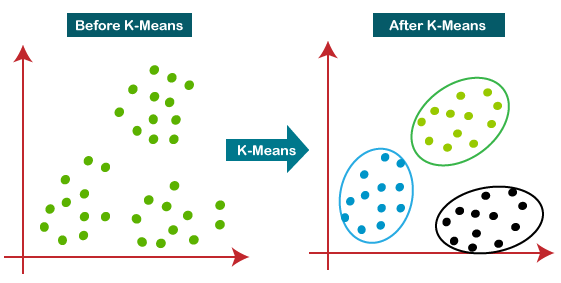
\includegraphics[width=0.7\textwidth]{images/kmeans.png}
    \caption{Set of data before and after the application of the K-Means algorithm}
    \label{fig:k_means}
\end{figure}


\subsection{Advantages and Limitations}
K-means is valued for its simplicity, efficiency, and scalability:
\begin{itemize}
    \item \textbf{Simplicity}: Easy to implement and interpret.
    \item \textbf{Efficiency}: Computationally efficient for moderate values of \( K \) and large datasets.
    \item \textbf{Versatility}: Applicable to a wide range of domains, including image compression and customer segmentation.
\end{itemize}


Despite its strengths, K-means has several limitations:
\begin{itemize}
    \item \textbf{Choice of \( K \)}: Requires prior knowledge of the number of clusters.
    \item \textbf{Initialization Sensitivity}: Poor initialization can lead to suboptimal clustering.
    \item \textbf{Cluster Shape Assumption}: Assumes clusters are spherical and of equal size, which may not hold for all datasets.
    \item \textbf{Outliers}: Sensitive to outliers, which can distort cluster centroids.
\end{itemize}

\subsection{Applications}

K-means clustering has numerous applications, including:
\begin{itemize}
    \item \textbf{Image Processing}: Color quantization and compression by reducing the number of colors in an image.
    \item \textbf{Market Segmentation}: Grouping customers based on purchasing behavior for targeted marketing.
    \item \textbf{Data Summarization}: Simplifying datasets by grouping similar data points.
    \item \textbf{Anomaly Detection}: Identifying outliers as data points that do not fit into any cluster well.
\end{itemize}

\subsection{Conclusion}

K-means clustering remains a foundational algorithm in machine learning due to its simplicity and effectiveness in solving clustering problems. While it has limitations, various extensions and initialization strategies, such as K-means++, have been developed to address these issues and improve the algorithm's robustness.


\section{Color Quantization}

Color quantization is a process used in image processing to reduce the number of distinct colors in an image while preserving its visual quality as much as possible. This is achieved by mapping the colors of the image to a smaller set of representative colors, known as a color palette. The result is a compressed image that retains its key visual features while using fewer colors.

\subsection{Purpose and Applications}

The main purpose of color quantization is to optimize image storage, processing, and transmission by reducing the complexity of the color information. It is widely used in several fields, including:

\begin{itemize}
    \item \textbf{Image Compression}: Reducing storage requirements for digital images by representing them with fewer colors.
    \item \textbf{Computer Graphics}: Rendering images efficiently on devices with limited color display capabilities.
    \item \textbf{Printing}: Mapping colors to a specific printer color gamut to ensure accurate reproduction.
    \item \textbf{Artistic Filters}: Creating stylized effects, such as cartoonization or posterization, by limiting the number of colors.
\end{itemize}

\subsection{Quantization Process}

The process of color quantization typically involves the following steps:

\begin{enumerate}
    \item \textbf{Color Space Selection}: Choose a color space (e.g., RGB, HSV, or CIE-Lab) for representing the image's pixel values. The choice of color space can influence the effectiveness of quantization, as some spaces better capture perceptual differences between colors.
    
    \item \textbf{Clustering of Colors}: Group similar colors into clusters. Each cluster represents a single color in the reduced palette. Clustering algorithms, such as K-means, are commonly used for this purpose. The goal is to minimize the perceptual difference between the original image and the quantized image.
    
    \item \textbf{Color Mapping}: Replace the original colors of the image with the nearest colors from the reduced palette. This step assigns each pixel in the image to the color of its cluster centroid.
\end{enumerate}

\begin{figure}[H]
    \centering
    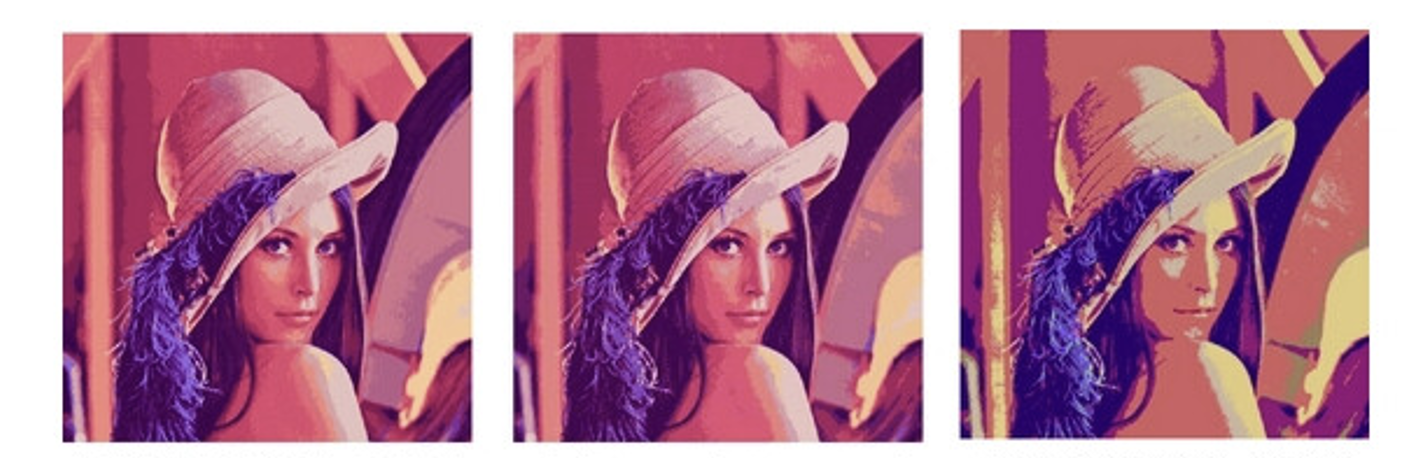
\includegraphics[width=0.7\textwidth]{images/color_quantization.png}
    \caption{Different color quantization algorithms applied to the same image}
    \label{fig:color_quantization}
\end{figure}

\subsection{Challenges in Color Quantization}

Color quantization is not without its challenges, which include:

\begin{itemize}
    \item \textbf{Perceptual Quality}: Reducing the number of colors can lead to visible artifacts or loss of detail, especially in images with subtle gradients.
    \item \textbf{Optimal Palette Selection}: Determining the optimal number and placement of colors in the palette is critical for balancing compression and visual fidelity.
    \item \textbf{Computational Cost}: Algorithms like K-means can be computationally expensive for high-resolution images, particularly with a large number of clusters.
    \item \textbf{Handling Outliers}: Outlier colors that do not belong to any major cluster can significantly affect the quality of the quantized image.
\end{itemize}


\subsection{Conclusion}

Color quantization is a crucial step in many image processing applications, balancing the trade-off between reducing storage requirements and maintaining visual quality. Techniques such as K-means clustering and median cut have been instrumental in achieving effective quantization, though challenges remain in optimizing perceptual quality and computational efficiency. In this work, color quantization plays a key role in achieving the desired cartoon-style effect by reducing the complexity of the image while preserving its essential features.


\chapter{Technologies}
\subsection{CUDA}

CUDA (Compute Unified Device Architecture) is a parallel computing platform and application programming interface (API) developed by NVIDIA. It enables developers to utilize the power of NVIDIA GPUs for general-purpose computing tasks. By leveraging CUDA, applications can perform computations faster by distributing tasks across thousands of GPU cores. It is widely used in fields such as scientific computing, machine learning, and real-time rendering.


\subsubsection{NVIDIA Nsight Compute}
NVIDIA Nsight Compute is a performance analysis tool designed for CUDA applications. It provides detailed metrics and insights into GPU kernel execution, enabling developers to identify bottlenecks and optimize their code. This tool is essential for understanding and improving the performance of GPU-accelerated applications.

\subsubsection{NVIDIA Nsight Systems}
NVIDIA Nsight Systems is a system-wide performance analysis tool that helps developers identify performance issues across the CPU and GPU. It provides a holistic view of application behavior, enabling optimization at both the system and application levels.

In the results section, we will analyze our findings using these tools to evaluate the performance of our CUDA-based implementations.

\subsection{OpenCV}

OpenCV (Open Source Computer Vision Library) is an open-source library designed for real-time computer vision and image processing tasks. It provides a wide range of tools and functions for image manipulation, feature extraction, object detection, and more. OpenCV is widely adopted in industries such as robotics, medical imaging, and autonomous vehicles due to its versatility and robust performance.

Some key features of OpenCV include:
\begin{itemize}
\item \textbf{Wide Functionality:} OpenCV supports tasks such as image filtering, geometric transformations, and object recognition.
\item \textbf{Cross-Platform Support:} OpenCV works on multiple platforms, including Windows, Linux, macOS, and Android.
\item \textbf{Hardware Acceleration:} OpenCV integrates with CUDA and OpenCL to accelerate processing on compatible hardware.
\end{itemize}

OpenCV is written in C++ but provides bindings for Python, Java, and other languages, making it accessible to a wide range of developers. With its comprehensive functionality and active community, OpenCV remains a cornerstone of computer vision development.


\chapter{Technical implementation}
In this chapter, we present an overview of our work on implementing k-means clustering algorithms for image processing. Two distinct approaches have been developed, each tailored to different computational paradigms and performance goals:

\begin{itemize}
\item \textbf{Sequential Algorithm:} A straightforward implementation in C++ that processes the input image using the k-means clustering technique. This version, while simple and easy to understand, is optimized for single-threaded execution and serves as a baseline for performance comparisons.
\item \textbf{Parallel Algorithm with CUDA:} A high-performance version of the k-means algorithm designed to utilize NVIDIA GPUs. This approach leverages CUDA to perform computations in parallel across thousands of GPU cores, providing significant speedups for large-scale image data.
\end{itemize}

These implementations highlight the trade-offs between simplicity and performance, and they serve as a foundation for evaluating the impact of parallelization on clustering algorithms. The following sections will delve into the specifics of each implementation, detailing their design, execution, and performance considerations.

\section{Sequential cartoonizer}
We will now break down and analyze different parts of the code, explaining how each segment works and contributes to the overall functionality of the cartoonizer.

\subsection{Euclidean Distance Function}
This function computes the Euclidean distance between two colors, which is essential for finding the nearest cluster centroid during the K-means algorithm.

\begin{lstlisting}[language=C++]
// Compute the Euclidean distance between two colors
float euclidean_distance(const Color& a, const Color& b) {
    return std::sqrt((a.r - b.r) * (a.r - b.r) + (a.g - b.g) * (a.g - b.g) + (a.b - b.b) * (a.b - b.b));
}
\end{lstlisting}

\textbf{Explanation:}
This function calculates the squared differences in the RGB values between two colors and returns the square root of the sum of those squared differences. This distance metric is used to compare how close two colors are in RGB space.

\subsection{Update Centroids Function}
After assigning each pixel to the nearest centroid, the centroids need to be updated by averaging the pixel colors assigned to each cluster.

\begin{lstlisting}[language=C++]
// Update centroids based on pixel assignments
void update_centroids(const std::vector<Color>& pixels, const std::vector<int>& assignments, std::vector<Color>& centroids, int k) {
    std::vector<int> cluster_sizes(k, 0);
    std::vector<Color> new_centroids(k, {0.0f, 0.0f, 0.0f});

    for (size_t i = 0; i < pixels.size(); i++) {
        int cluster_idx = assignments[i];
        new_centroids[cluster_idx].r += pixels[i].r;
        new_centroids[cluster_idx].g += pixels[i].g;
        new_centroids[cluster_idx].b += pixels[i].b;
        cluster_sizes[cluster_idx]++;
    }

    for (int i = 0; i < k; i++) {
        if (cluster_sizes[i] > 0) {
            new_centroids[i].r /= cluster_sizes[i];
            new_centroids[i].g /= cluster_sizes[i];
            new_centroids[i].b /= cluster_sizes[i];
        }
    }

    centroids = new_centroids;
}
\end{lstlisting}

\textbf{Explanation:}
This function iterates over each pixel and updates the centroids by averaging the colors of all pixels assigned to each cluster. It ensures that the new centroids represent the average color of each cluster, which will be used in the next iteration.

\subsection{K-means Function}
The main function implementing the K-means algorithm for color quantization. It converts the image to a set of color values, applies the K-means clustering algorithm, and then generates the output image with reduced colors.

\begin{lstlisting}[language=C++]
// K-means algorithm for color quantization
void kmeans_cpu(const cv::Mat& image, int k, int max_iter, cv::Mat& output_image,int seed) {
    int width = image.cols;
    int height = image.rows;
    int num_pixels = width * height;

    // Convert image to a vector of Color structs
    std::vector<Color> pixels(num_pixels);
    for (int i = 0; i < height; i++) {
        for (int j = 0; j < width; j++) {
            cv::Vec3b color = image.at<cv::Vec3b>(i, j);
            pixels[i * width + j] = { color[2] / 255.0f, color[1] / 255.0f, color[0] / 255.0f };
        }
    }

    srand(seed);

    // Randomly initialize centroids
    std::vector<Color> centroids(k);
    for (int i = 0; i < k; i++) {
        centroids[i] = { float(rand()) / RAND_MAX, float(rand()) / RAND_MAX, float(rand()) / RAND_MAX };
    }

    std::vector<int> assignments(num_pixels, 0);
    for (int iter = 0; iter < max_iter; iter++) {
        // Step 1: Assign each pixel to the closest centroid
        for (int i = 0; i < num_pixels; i++) {
            float min_dist = std::numeric_limits<float>::max();
            for (int j = 0; j < k; j++) {
                float dist = euclidean_distance(pixels[i], centroids[j]);
                if (dist < min_dist) {
                    min_dist = dist;
                    assignments[i] = j;
                }
            }
        }

        // Step 2: Update centroids based on the pixel assignments
        update_centroids(pixels, assignments, centroids, k);
    }

    // Step 3: Create the output image
    output_image = image.clone();
    for (int i = 0; i < height; i++) {
        for (int j = 0; j < width; j++) {
            int cluster_idx = assignments[i * width + j];
            cv::Vec3b new_color(
                static_cast<unsigned char>(centroids[cluster_idx].b * 255),
                static_cast<unsigned char>(centroids[cluster_idx].g * 255),
                static_cast<unsigned char>(centroids[cluster_idx].r * 255)
            );
            output_image.at<cv::Vec3b>(i, j) = new_color;
        }
    }
}
\end{lstlisting}

\textbf{Explanation:}
- The function first converts the input image into a vector of `Color` structs. Each pixel’s RGB values are normalized between 0 and 1.
- It randomly initializes the centroids, assigns each pixel to the nearest centroid, and updates the centroids in each iteration.
- After \( \text{max\_iter} \) iterations, the final output image is generated where each pixel is replaced by the corresponding centroid color.

\subsection{Main Function}
The main driver code calls the functions, loads the image, applies K-means, and saves the output image.

\begin{lstlisting}[language=C++]
int main(int argc, char* argv[]) {
    int clusters = DEFAULT_CLUSTERS;
    int iterations = DEFAULT_ITERATIONS;
    int seed = DEFAULT_SEED;
    int threads_per_block = DEFAULT_THREADS;
    std::string input_image_path = "images/image.jpg";
    std::string output_image_path = "images/cartoon_cpu.jpg";

    arg_parser(argc, argv, clusters, iterations, seed, threads_per_block, input_image_path, output_image_path);

    // Load the image
    cv::Mat image = cv::imread(input_image_path);
    if (image.empty()) {
        std::cerr << "Error loading image!" << std::endl;
        return -1;
    }

    cv::Mat output_image;
    kmeans_cpu(image, clusters, iterations, output_image, seed);

    // Save the output
    cv::imwrite(output_image_path, output_image);
    std::cout << "CPU output saved!" << std::endl;
    return 0;
}
\end{lstlisting}

\textbf{Explanation:}
The main function reads the input image, applies the K-means algorithm, and saves the result as the output image.

\subsection{Conclusion}
The K-means algorithm used in this code provides an effective way to reduce the color complexity of an image, giving it a cartoon-like appearance. By analyzing and applying clustering to pixel colors, the image becomes more abstract and simplified, which enhances the cartoon effect.



\section{Parallel cartoonizer}

\printbibliography
\end{document}  % Fine del documento